%%%%%%%%%%%%%%%%%%%%%%%%%%%%%%%%%%%%%
%                                   %
% Compile with XeLaTeX and biber    %
%                                   %
% Questions or comments:            %
%                                   %
% joshua dot mcneill at uga dot edu %
%                                   %
%%%%%%%%%%%%%%%%%%%%%%%%%%%%%%%%%%%%%

\documentclass{beamer}
  % Read in standard preamble (cosmetic stuff)
  %%%%%%%%%%%%%%%%%%%%%%%%%%%%%%%%%%%%%%%%%%%%%%%%%%%%%%%%%%%%%%%%
% This is a standard preamble used in for all slide documents. %
% It basically contains cosmetic settings.                     %
%                                                              %
% Joshua McNeill                                               %
% joshua dot mcneill at uga dot edu                            %
%%%%%%%%%%%%%%%%%%%%%%%%%%%%%%%%%%%%%%%%%%%%%%%%%%%%%%%%%%%%%%%%

% Beamer settings
% \usetheme{Berkeley}
\usetheme{CambridgeUS}
% \usecolortheme{dove}
% \usecolortheme{rose}
\usecolortheme{seagull}
\usefonttheme{professionalfonts}
\usefonttheme{serif}
\setbeamertemplate{bibliography item}{}

% Packages and settings
\usepackage{fontspec}
  \setmainfont{Charis SIL}
\usepackage{hyperref}
  \hypersetup{colorlinks=true,
              allcolors=blue}
\usepackage{graphicx}
  \graphicspath{{../../figures/}}
\usepackage[normalem]{ulem}
\usepackage{enumerate}

% Document information
\author{M. McNeill}
\title[FREN2001]{Français 2001}
\institute{\url{joshua.mcneill@uga.edu}}
\date{}

%% Custom commands
% Lexical items
\newcommand{\lexi}[1]{\textit{#1}}
% Gloss
\newcommand{\gloss}[1]{`#1'}
\newcommand{\tinygloss}[1]{{\tiny`#1'}}
% Orthographic representations
\newcommand{\orth}[1]{$\langle$#1$\rangle$}
% Utterances (pragmatics)
\newcommand{\uttr}[1]{`#1'}
% Sentences (pragmatics)
\newcommand{\sent}[1]{\textit{#1}}
% Base dir for definitions
\newcommand{\defs}{../definitions}


  % Packages and settings

  % Document information
  \subtitle[Casse-croûtes et articles]{Les casse-croûtes et les articles}

\begin{document}
  % Read in the standard intro slides (title page and table of contents)
  \begin{frame}
    \titlepage
    \tiny{Office: % Basically a variable for office hours location
Gilbert 121\\
          Office hours: % Basically a variable for office hours
 lundi, mercredi, vendredi 10:10--11:10
}
  \end{frame}

  \begin{frame}{}
    \begin{center}
      \Large Quiz
    \end{center}
  \end{frame}

  \begin{frame}{Les articles}
    \begin{columns}
      \column{0.55\textwidth}
        Qu'est-ce que cette personne prend ou boit?
        \begin{enumerate}
          \item<2-> Dale Cooper boit du café.
          \item<2-> \emph{Est-ce qu'il boit du thé?}
          \item<3-> Non, il ne boit pas de thé.
          \item<3-> \emph{Est-ce qu'il boit de la limonade?}
          \item<4-> Non, il ne boit pas de limonade.
        \end{enumerate}
      \column{0.45\textwidth}
        \begin{minipage}[c][0.6\textwidth]{\linewidth}
          \begin{center}
            \only<-4>{
              
\includegraphics[scale=0.15]{coffee.png}
            }
          \end{center}
        \end{minipage}
    \end{columns}
  \end{frame}

  \begin{frame}{Les articles}
    \begin{columns}
      \column{0.55\textwidth}
        Qu'est-ce que cette personne mange ou boit?
        \begin{enumerate}
          \item<2-> Kourtney mange de la salade verte.
          \item<2-> \emph{Est-ce qu'elle mange de la salade composée?}
          \item<3-> Non, elle ne mange pas de salade composée.
          \item<3-> \emph{Est-ce qu'elle mange un croque-madame?}
          \item<4-> Non, elle ne mange pas de croque-madame.
        \end{enumerate}
      \column{0.45\textwidth}
        \begin{minipage}[c][0.6\textwidth]{\linewidth}
          \begin{center}
            \only<-4>{
              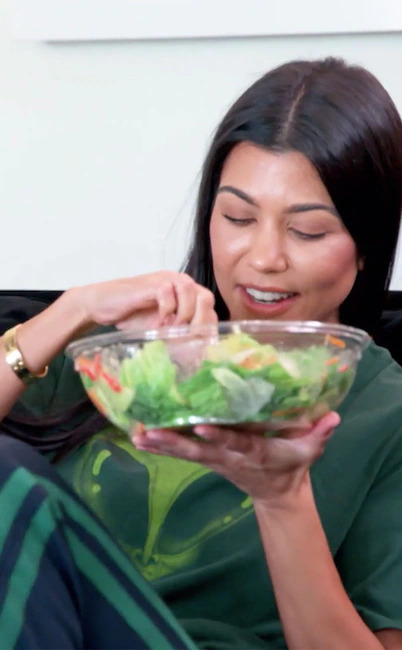
\includegraphics[scale=0.27]{salade.jpg}
            }
          \end{center}
        \end{minipage}
    \end{columns}
  \end{frame}

  \begin{frame}{Les articles}
    \begin{columns}
      \column{0.55\textwidth}
        Qu'est-ce que cette personne prend ou boit?
        \begin{enumerate}
          \item<2-> Jon Stewart mange de la pizza.
          \item<2-> \emph{Est-ce qu'il mange des sandwichs au jambon?}
          \item<3-> Non, il ne mange pas de sandwichs au jambon.
          \item<3-> \emph{Est-ce qu'il mange un croque-monsieur?}
          \item<4-> Non, il ne mange pas de croque-monsieur.
        \end{enumerate}
      \column{0.45\textwidth}
        \begin{minipage}[c][0.6\textwidth]{\linewidth}
          \begin{center}
            \only<-4>{
              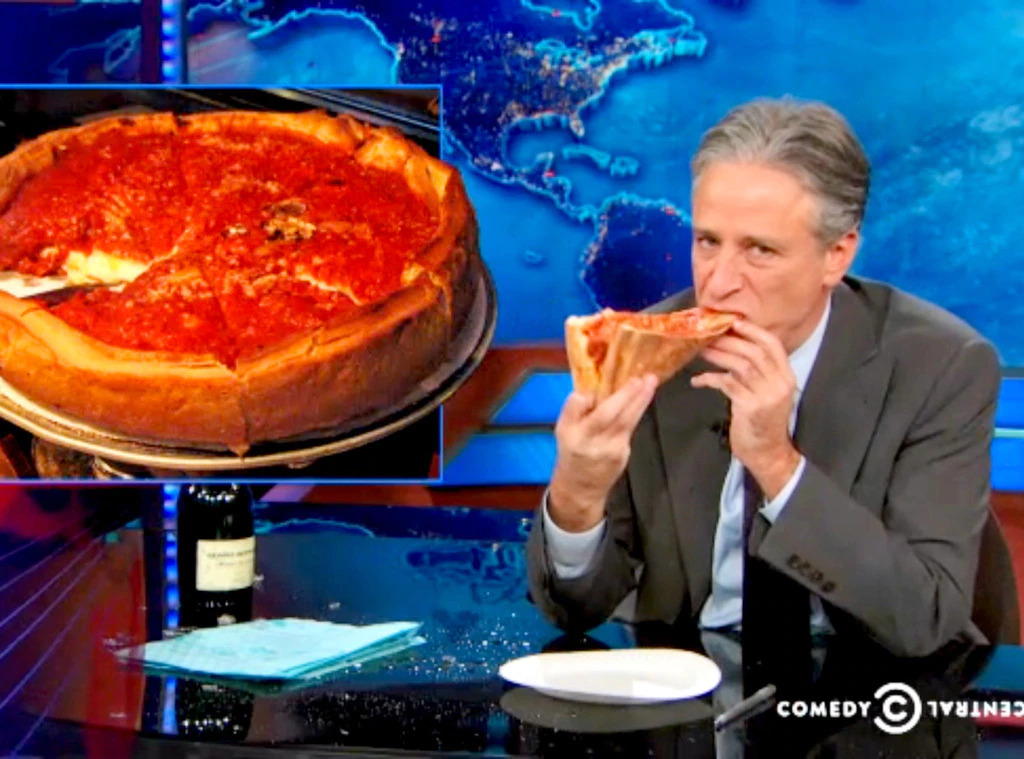
\includegraphics[scale=0.15]{pizza.jpg}
            }
          \end{center}
        \end{minipage}
    \end{columns}
  \end{frame}

  % \begin{frame}{Les articles}
  %   \begin{columns}
  %     \column{0.55\textwidth}
  %       Qu'est-ce que cette personne prend ou boit?
  %       \begin{enumerate}
  %         \item<2-> Le Governator mange de la glace.
  %         \item<2-> \emph{Est-ce qu'il mange un sandwich au jambon?}
  %         \item<3-> Non, il ne mange pas de sandwich au jambon.
  %         \item<3-> \emph{Est-ce qu'il mange un sandwich au fromage?}
  %         \item<4-> Non, il ne mange pas de sandwich!
  %       \end{enumerate}
  %     \column{0.45\textwidth}
  %       \begin{minipage}[c][0.6\textwidth]{\linewidth}
  %         \begin{center}
  %           \only<-4>{
  %             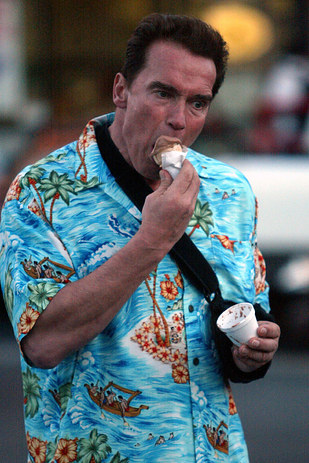
\includegraphics[scale=0.35]{glace.jpg}
  %           }
  %         \end{center}
  %       \end{minipage}
  %   \end{columns}
  % \end{frame}

  \begin{frame}{Les articles}
    \begin{columns}
      \column{0.5\textwidth}
        Qu'est-ce que ces personnes prennent ou boivent?
        \begin{enumerate}
          \item<2-> Ils boivent du thé.
          \item<2-> \emph{Est-ce qu'ils boivent du chocolat chaud?}
          \item<3-> Non, ils ne boivent pas de chocolat chaud.
          \item<3-> \emph{Est-ce qu'ils boivent du thé glacé?}
          \item<4-> Non, ils boivent du thé chaud!
        \end{enumerate}
      \column{0.45\textwidth}
        \begin{minipage}[c][0.6\textwidth]{\linewidth}
          \begin{center}
            \only<-4>{
              \includegraphics[scale=0.15]{thé.png}
            }
          \end{center}
        \end{minipage}
    \end{columns}
  \end{frame}

  \begin{frame}{Qu'est-ce que tu prends?}
    Avec un/e partenaire, parle de ce que tu prends pour manger ou boire dans les situations suivantes. \\
    \tinygloss{With a partner, talk about what you have to eat or drink in the following situations.}
    \begin{description}
      \item[] \textbf{Modèle:} \emph{Tu es au régime.}
      \item[E1:] Moi, je mange une salade verte.
      \item[E2:] Pour moi, j'ai plus faim, alors je prends une salade composée.
    \end{description}
    \begin{columns}[t]
      \column{0.5\textwidth}
        \begin{enumerate}
          \item Tu es au café.
          \item Tu as du mal à te réveiller.
          \item Tu as envie d'une boisson chaude.
          \item Tu aimes pas le sucre.
        \end{enumerate}
      \column{0.5\textwidth}
        \begin{enumerate}
          \setcounter{enumi}{4}
          \item Tu regardes la télé.
          \item Tu n'as pas le temps de manger.
          % \item Tu sors avec des amis.
          \item Tu ne peux pas dormir.
          \item Tu as très soif.
        \end{enumerate}
    \end{columns}
  \end{frame}

  \begin{frame}{Prendre les commandes}

    {\small Placez-vous en groupes de 4.
    Chaque groupe représente une table à un café.
    Une personne de chaque groupe va être un/e serveur/-euse qui prend les commandes d'un autre groupe, et une autre va être un chef qui sert les aliments.
    Les commandes consistent d'une \alert{boisson} et d'un \alert{aliment} au moins.
    Enfin, le/la serveur/-euse va donner les commandes aux chefs qui vont les servir.} \\

    \tinygloss{Form 4 groups.
    Each group represents a table at a cafe.
    One person from each group will be a waitor/-tress who takes the orders of another group, and another will be a chef who serves the food.
    The orders consist of a \alert{drink} and \alert{food} at least.
    Finally, the waitors/-tresses will give the orders to the chefs who will serve them.}
    \begin{description}
      \small
      \item[] \textbf{Modèle:}
      \item[E1:] (serveur/-euse) Je suis votre serveur/-euse. Qu'est-ce que vous prenez?
      \item[E2:] Moi, je voudrais du café, un croque-monsieur et des frites.
      \item[E3:] Pour moi, une salade verte et de l'eau sans glaçons. Je suis au régime!
      \item[E4:] (chef) Qui prend le croque-monsieur, les frites et le café?
    \end{description}
  \end{frame}

  \begin{frame}{}
    \begin{center}
      \Large Questions?
    \end{center}
  \end{frame}
\end{document}
